

\chapter{Sistema de controlo e monitorização}


Este capítulo tem como objetivo a descrição do sistema que resultou do trabalho prático
desta dissertação. Para esse fim, cada elemento pertencente ao sistema é caracterizado de
acordo com as suas funções e especificidades. É também descrito como os elementos interagem
entre si.


%Tendo como base, por um lado os resultados da pesquisa efectuada em 2003 e, por outro lado, as indicações e expectativas fornecidas pelos representantes da Liftech, empresa que actua neste projecto como o cliente do produto a desenvolver, foi elaborada a especificação funcional do sistema.

%Neste capítulo são descritos separadamente cada um dos módulos que compõem o sistema, quer ao nível da sua arquitectura, quer ao nível do software de suporte.



%Dashboard - Interface que apresenta a informação mais importante para o utilizador de forma apelativa, tornando mais fácil a interacção e respetiva leitura


% Mockups - Design que a plataforma deverá apresentar no fim do seu desenvolvimento.


\section{Descrição global do sistema}


Este sistema tem como objetivo a supervisão remota da produção de salicornia,  permitindo não só a monitorização dos dados adquiridos pelos sensores, como também da atuação remota de determinados comandos. Neste contexto também será possível a aquisição de imagens que possibilitará a deteção de intrusos nas quintas onde se produz esta espécie.

O esquema da figura X ilustra todos os componentes de um modo geral e as diferentes plataformas com que o cliente pode interagir. 


%A figura 4.1 representa o diagrama de blocos do sistema, onde se encontram todos os seus elementos, seguidamente descritos.




\begin{figure}[!htb]
	\centering
	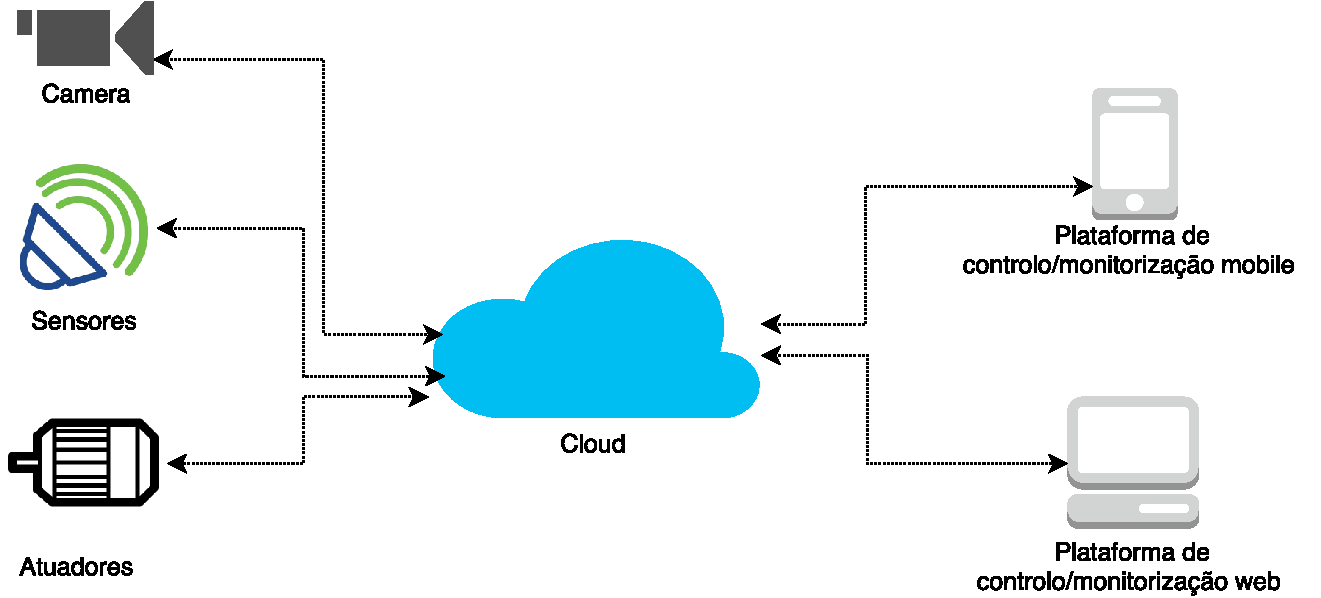
\includegraphics[scale=0.45]{esquemas/global_arquitetura.pdf}
	\caption{Ilustração principais componentes}
	\label{dikw}
\end{figure}







Como vimos no capitulo 3, uma plantação de  salicórnia carece de um controlo relativamente fino da salinidade do terreno onde ela cresce. A salinidade do terreno depende, por sua vez, das chuvas, da salinidade da água dos canais da ria, etc. Nas “quintas” de salicórnia da Ria, a produção faz-se numa espécie de leiras limitadas por pequenos canais de irrigação. Esses canais podem ser cheios de água salgada proveniente dos esteiros que rodeiam a “quinta”. Essa operação implica a abertura de válvulas de admissão dessa água, medida do nível da maré nos canais, monitorização da qualidade e salinidade da água exterior.
Por sua vez, a cultura pode ser ameaçada por excesso de água doce de chuvas ou ser objeto de vandalismo.


\begin{figure}[!htb]
	\centering
	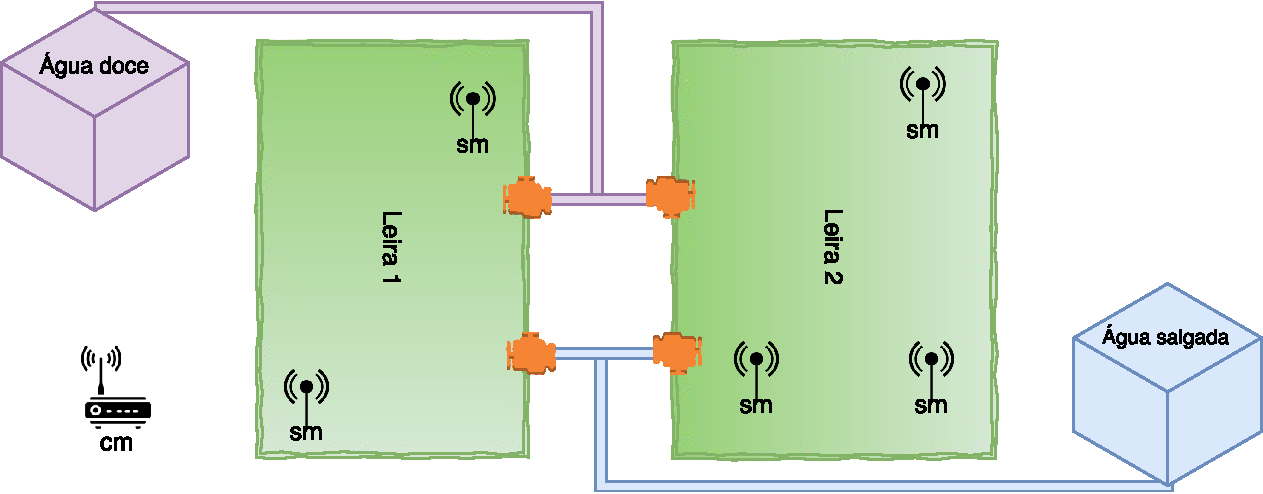
\includegraphics[scale=0.55]{esquemas/leiras-comm-geral.pdf}
	\caption{Ilustração de uma "quinta" onde se produz salicornia}
	\label{dikw}
\end{figure}





Neste contexto, cada grupo de sensores espalhado por cada leira irá comunicar com um módulo central, originando uma topologia de rede em estrela.  Por sua vez, este módulo irá comunicar diretamente com a servidor que possibilitará que os dados sejam tratados e disponíveis para visualização ao cliente.  Pressupõe-se portanto que este ultimo módulo tenha necessariamente ligação à rede wifi de modo a conseguir consumir a API REST desenvolvida para o efeito. 


\section{Componentes}

No contexto desta dissertação é necessário reter dois conceitos principais, são eles: 

\begin{itemize}
	\item \textbf{\textit{\ac{SM}}:} consiste num microcontrolador responsável pela aquisição de dados provenientes dos mais diversos tipos de sensores. Cada \textit{sensor module} terá que utilizar um determinado módulo de comunicação de modo a possibilitar a comunicação com o módulo central, sendo que este envia os dados adquiridos para o servidor. Para além disso, pretende-se que o sensor module possa ter controlo sobre si, ou seja, inteligência própria.  
	 
	\item \textbf{\textit{\ac{CM}}:} consiste num microcontrolador responsável pela recepção dos dados preveniente dos \textit{sensor modules}. Pretende-se que este módulo envie informações para os sensores modules quando requisitados pelo utilizador. 
	
	
	Não é mais do que um modulo central que recebe todos as...
\end{itemize}




A figura seguinte, ilustra a comunicação entre três \ac{SM} com um \ac{CM}. 


\begin{figure}[h]
	\centering
	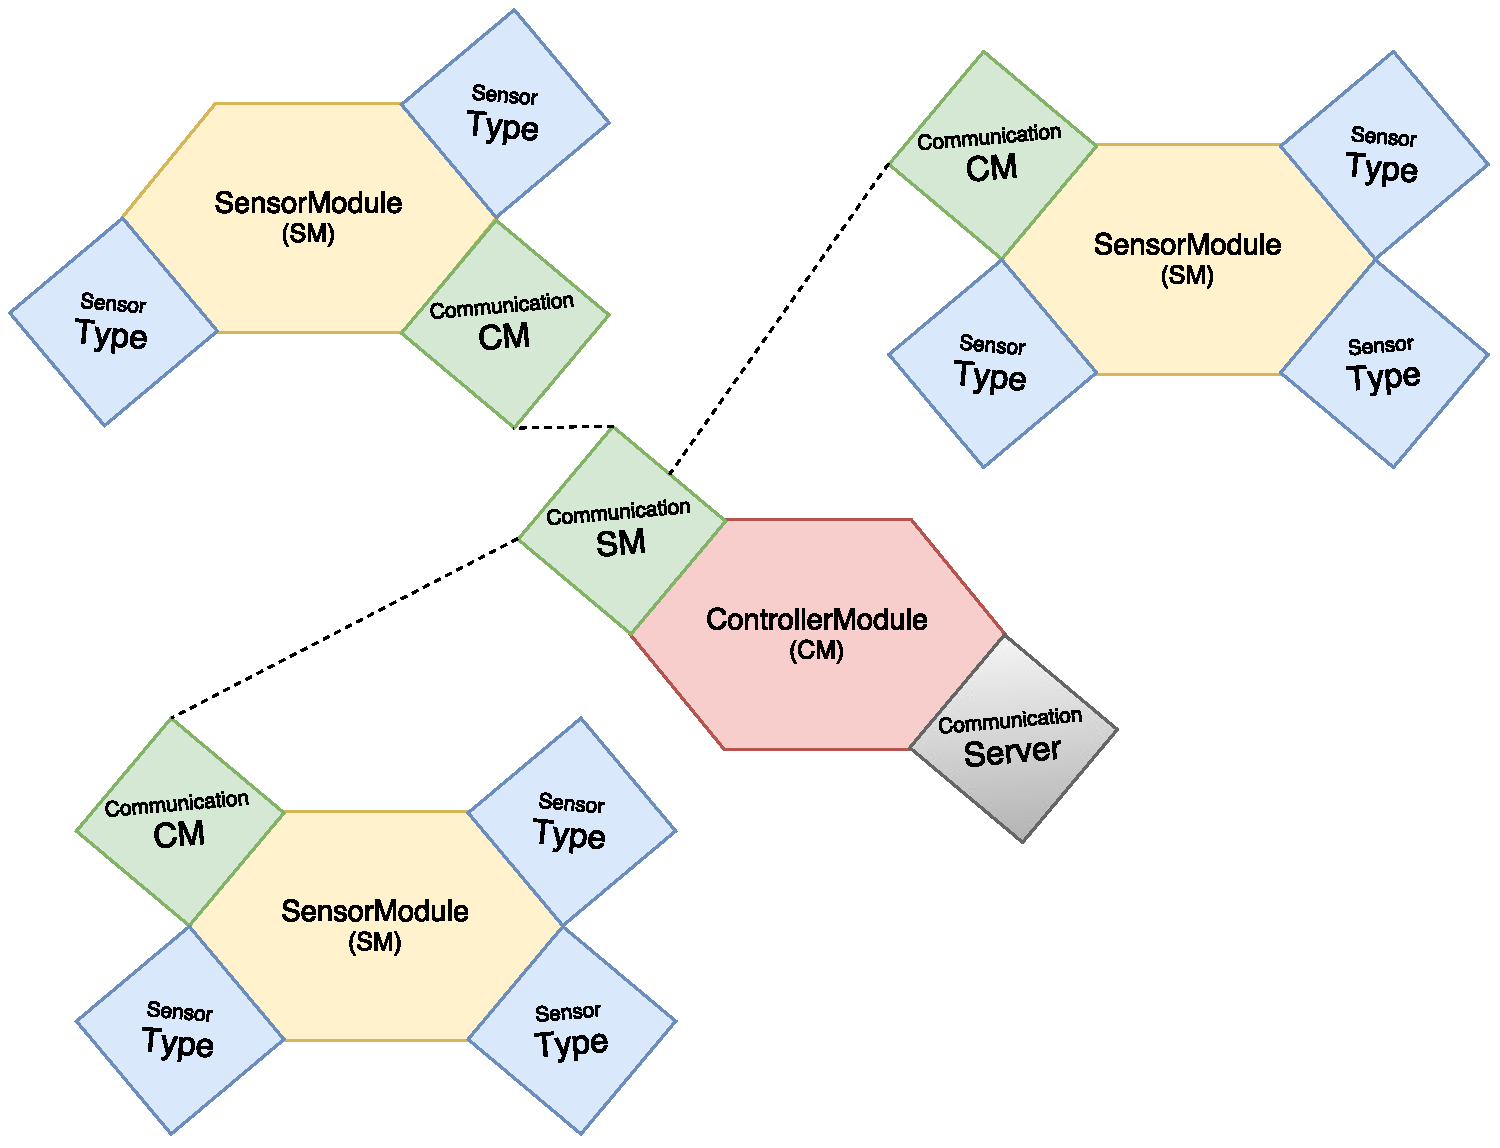
\includegraphics[scale=0.35]{esquemas/general-electronic-modules.pdf}
	\caption{Pirâmide do conhecimento: modelo DIKW}
	\label{dikw}
\end{figure}




\subsection{Controller Module}


\subsection{Sensor Module}









\newpage

\section{Design funcional}










\subsection{Requisitos funcionais}


%Os requisitos funcionais especificam os critérios que devem ser usados ​​para avaliar comportamentos ou funções especificas do sistema. Estes são os requisitos funcionais do sistema proposto nesta dissertação. 





\subsubsection{Dashboard}


\begin{itemize}
	\item A interface do sistema deve permitir que o usuário faça login no sistema
	Admin ou um usuário.
	
	\item A interface do sistema deve permitir que o usuário saia do sistema.
	
	\item O sistema deve permitir o armazenamento de informações do cliente.
	
	\item O sistema deve permitir a atualização das informações do cliente.
\end{itemize}


\subsubsection{Aplicação mobile}





\subsection{Requisitos não funcionais}


Requisitos não funcionais são todos os requisitos da aplicação relacionados com
performance, escalabilidade, segurança, disponibilidade e usabilidade. Estes não são
necessariamente pedidos pelo cliente. 


\begin{itemize}
	\item  o sistema deverá executar em qualquer plataforma.
	
	\item O sistema deverá disponibilizar uma API para que possam ser criados novos produtos com base neste 
	
	\item 
	
\end{itemize}







\section{Design técnico}



\subsection{Arquitetura do sistema}



\subsubsection{Camada de apresentação}


\subsubsection{Camada de negócio}



\subsubsection{Camada de dados}




\section{Diagrama de componentes}




\section{Sistema de interação}


\section{Descrição}


Modulos da daniela : Cc1110



\section{Arquitetura geral}




\newpage












\section{Considerações finais}